\documentclass{article}
\usepackage[UTF8]{ctex}
% Replace `letterpaper' with`a4paper' for UK/EU standard size
\usepackage[a4paper,top=2cm,bottom=2cm,left=3cm,right=3cm,marginparwidth=1.75cm]{geometry}

% Useful packages
\usepackage{amsmath}
\usepackage{graphicx}
\usepackage[colorlinks=true, allcolors=blue]{hyperref}
\usepackage{graphicx} %插入图片的宏包
\usepackage{float} %设置图片浮动位置的宏包
\usepackage{subfigure} %插入多图时用子图显示的宏包
\usepackage{parskip}
\usepackage{indentfirst} 
\setlength{\parindent}{2em}
\usepackage{hyperref}  
\usepackage{tikz}
\allowdisplaybreaks
\usepackage{multirow}
\usepackage{amsmath}
\usepackage{amsfonts,amssymb} 
\usepackage{xcolor} % 用于显示颜色
\usepackage{listings} % 用于插入代码
\usepackage{tikz} % 导入多重比较示意图专用
\usetikzlibrary{decorations,arrows,shapes} % 导入多重比较示意图专用

\lstset{
	basicstyle          =   \sffamily,          % 基本代码风格
	keywordstyle        =   \bfseries,          % 关键字风格
	commentstyle        =   \rmfamily\itshape,  % 注释的风格,斜体
	stringstyle         =   \ttfamily,  % 字符串风格
	flexiblecolumns,                % 别问为什么,加上这个
	numbers             =   left,   % 行号的位置在左边
	showspaces          =   false,  % 是否显示空格,显示了有点乱,所以不现实了
	numberstyle         =   \zihao{-5}\ttfamily,    % 行号的样式,小五号,tt等宽字体
	showstringspaces    =   false,
	captionpos          =   t,      % 这段代码的名字所呈现的位置,t指的是top上面
	frame               =   lrtb,   % 显示边框
}

\lstdefinestyle{R}{
	language        =   R, % 语言选R
	basicstyle      =   \zihao{-5}\ttfamily,
	numberstyle     =   \zihao{-5}\ttfamily,
	keywordstyle    =   \color{blue},
	keywordstyle    =   [2] \color{teal},
	stringstyle     =   \color{magenta},
	commentstyle    =   \color{red}\ttfamily,
	breaklines      =   true,   % 自动换行,建议不要写太长的行
	columns         =   fixed,  % 如果不加这一句,字间距就不固定,很丑,必须加
	basewidth       =   0.5em,
}

\lstdefinestyle{Python}{
	language        =   Python, % 语言选R
	basicstyle      =   \zihao{-5}\ttfamily,
	numberstyle     =   \zihao{-5}\ttfamily,
	keywordstyle    =   \color{blue},
	keywordstyle    =   [2] \color{teal},
	stringstyle     =   \color{magenta},
	commentstyle    =   \color{red}\ttfamily,
	breaklines      =   true,   % 自动换行,建议不要写太长的行
	columns         =   fixed,  % 如果不加这一句,字间距就不固定,很丑,必须加
	basewidth       =   0.5em,
}

\title{基于Wald检验、逻辑回归、多重填补、条件把握度、$\alpha$消耗函数、Graphical Approach和广义估计方程等多种统计方法的三期临床试验数据分析报告}
\author{}
\date{}

\begin{document}
	\maketitle
	\tableofcontents

\section{问题一}
\subsection{问题1.1}
根据ICH E9(R1)的有关定义,我们提出的估计目标为:
在满足入排标准的人群中,较安慰剂组而言,
该药物在第24周时通过患者评分标准A判定的疾病较基线的改善情况。

该估计目标的五个属性如下:
\begin{enumerate}
    \item 治疗:受试者从第0周开始每隔4周
    到研究中心进行给药并接受定期检查。
    \item 人群:满足入排标准,经过分层随机分配到
    药物组和安慰剂组的所有受试者。
    \item 变量:受试者在第24周时通过患者评分标准A
    判定的疾病较基线是否改善(二分类变量)。
    \item 伴发事件:1)患者在24周前终止治疗并退出试验;
    2)患者在24周之内采取了额外治疗,如背景治疗改变、补救治疗等。
    \item 群体层面汇总:统计药物组和安慰剂组在第24周时
    经患者评分标准A判定为疾病较基线有所改善的受试者比例(以下简称应答率),
    并求出两组间应答率差值的95$\%$可信区间。
\end{enumerate}

该估计目标较为合理,因为该目标能精确描述
为实现研究目标而需要估计的治疗效应,并在群体水平上
汇总比较同质性患者在不同治疗条件下的结局,
能够反映出该药物相比于安慰剂在治疗有效性和安全性上的差异。

\subsection{问题1.2}
根据问题1.1所述估计目标,我们认为这是一个对二分类资料
的分析问题。

首先,应采用\textbf{卡方检验},
根据两组受试者中应答者和非应答者数量列出四格表如下:
\begin{table}[H]
    \centering
    \begin{tabular}{llll}
    \hline
         & 无应答 & 应答 &   合计      \\ 
    \hline
    安慰剂组 & a    & b    & a+b     \\
    药物组  & c    & d    & c+d     \\
    \hline
     合计    & a+c  & b+d  & a+b+c+d \\ 
    \hline
    \end{tabular}
    \end{table}
通过计算对应的p值,可以检测药物组和安慰剂组
的应答率差异是否具有统计学意义。

其次,可以借助\textbf{Wald test},估计两组应答率的差异。
对于总体应答率$\pi$而言,当样本量$n$足够大,样本应答率率$P$不太小,$(1-P)$也不会太小,
比如$n(1-P)P>5$时,根据中心极限定理,$P$的抽样分布可以用正态分布近似,也即:
\[P\to \mathcal{N} (\pi,\frac{P(1-P)}{n})\]

记$P_0, P_1$分别为安慰剂组和药物组的样本应答率,那么
\[ S_0 = \sqrt{\frac{P_0(1-P_0)}{n_0}},\, S_1 = \sqrt{\frac{P_1(1-P_1)}{n_1}}\]
分别为安慰剂组与药物组的样本应答率的标准误。根据概率论的知识,当两组样本量比较大时,
两组的比例差异近似于服从下述正态分布:
\[P_1 - P_0 \to \mathcal{N} (\pi_1-\pi_0, S_0^2 + S_1^2)\]
进一步可以使用单侧的Wald test,检测安慰剂组和药物组的应答率的差异是否有统计学意,
并估计两组应答率差值的95$\%$置信区间为:
\[ P_1-P_0 \pm Z_{\alpha/2}\sqrt{ S_0^2 + S_1^2} \]


再者,也可以考虑建立\textbf{多元逻辑回归模型}。
以分组(药物组、安慰剂组)作为自变量,
考虑到分层因素,可以再加入所在中心(亚洲、欧洲、北美洲)和
体重(轻重)作为协变量,建立多元逻辑回归模型如下:
\begin{align*}
    \log\left(\frac{p_i}{1-p_i}\right) =
    \beta_0 + \beta_1 X_1 + \beta_2 X_2 + \beta_3 X_3 + \beta_4 X_4
\end{align*}
\par 其中:
\par $X_1$:表示体重,0表示对应基线体重为轻,1表示对应基线体重为重。
\par $X_2,X_3$:表示地区,$X_2=0,X_3=0$表示亚洲,
    $X_2=1,X_3=0$表示欧洲,$X_2=0,X_3=1$表示北美洲。
\par $X_4$:表示分组,0表示安慰剂组,1表示药物组。

然后再通过逐步回归的方法,去除影响不显著的变量。
该模型能够排除地区和体重所带来的干扰。此外,
$\exp(\beta_4)$ 即为对应于受试者分组的的优势比$OR_4$。当该优势比
大于1的时候,可以认为药物组相较于安慰剂组确实更有效。由于$\beta_4$
是未知参数,可以基于观察数据结合模型
求出$\beta_4$的估计值$b_4$和标准误$Se(b_4)$,
得到对应于分组情况$X_4$的总体优势比$OR_4$的$1-\alpha$可信区间
\[ \exp \left[ b_j \pm Z_{\alpha/2} Se(b_j) \right]\]

\subsection{问题1.3}
我们假定数据缺失机制为MAR。
我们认为,可以使用多重逻辑回归填补法对缺失数据进行填补。
先用所有在第24周观测到的数据,得到问题1.2中提出的逻辑回归模型。
将每个缺失第24周数据的受试者体重、地区和所在组别带入模型,
求出其第24周应答的概率$P$,再生成多个
应答率为$P$的服从伯努利分布随机数,作为该缺失者的多个填补值,
从而得到多个填补后的完整数据集。
然后,使用鲁宾法则,将各数据集的结果汇总,
得到最终的两组应答率之差的估计值、标准误、
置信区间,以及用填补数据拟合出的多元逻辑回归模型。
将这些填补后所得结果与未考虑缺失数据所得结果
进行比较,若二者接近,则可以证明主要分析结果的稳健性。以上填补过程可以使用
R语言中的mice包完成。

我们认为,这种基于多重逻辑回归的后验填补方法,
可以保证结果具有较小的偏差和较大的有效性。

至于临界点方法,应往“对原分析结果更不利”的方向考虑,
假设药物组和安慰剂组中退出试验的受试者
的应答率,然后计算在该应答率下的
假设检验结果,在本题中,即为卡方检验是否有显著性差异,
以及两组样本应答率之差的置信区间是否包含0。我们分别调整
两组中提前退出的受试者的应答率,找到使得上述检验结果发生反转
的临界值,这个临界值就是一个临界点。由于我们允许两组中假设的
提前退出者的应答率可以不同,因此应该有不止一个临界点,我们推测临界点
应分布于某条曲线附近。
\subsection{问题1.4}
首先,我们对未缺失部分的数据进行卡方检验,列出四格表如下:
\begin{table}[H]
    \centering
    \begin{tabular}{llll}
        \hline
         & 无应答 & 应答 & 合计  \\
         \hline
    药物组  & 33   & 52   & 85  \\
    安慰剂组 & 55   & 30   & 85  \\
    \hline
    合计   & 88   & 82   & 170\\
    \hline
    \end{tabular}
    \end{table}
利用R语言进行Yates'连续性校正后的卡方检验,结果为
\[\chi^2=10.389,\,p=0.001267<0.05\] 按$\alpha=0.05$
的水准拒绝原假设,差别有统计学意义,可以认为药物组应答率
高于安慰剂组。

下面,我们近似估计两组应答率之差的置信区间。
由上述四格表可知:
\begin{align*}
    P_0 &= \frac{30}{85} = 0.3529 \\
    P_1 &= \frac{52}{85} = 0.6118 \\
    P_1-P_0 &= 0.6118-0.3529=0.2589\\
    S_0 & = \sqrt{\frac{P_0(1-P_0)}{n_0}} = 0.05183\\
    S_1 & = \sqrt{\frac{P_1(1-P_1)}{n_1}} =  0.05286\\
    S &= \sqrt{ S_0^2 + S_1^2}\\
      &= \sqrt{0.05183^2 + 0.05286^2} \\
      &=0.07403\\
    CI_{0.95} &= P_1-P_0 \pm Z_{\alpha/2}\sqrt{ S_0^2 + S_1^2}\\
    =& (0.1137, 0.4039)
\end{align*}
注意到95$\%$置信区间不包含0,这等价于按$\alpha=0.05$
的水准拒绝原假设,可以认为药物组应答率高于安慰剂组。

最后,我们对未缺失的数据进行逻辑回归分析,并进行逐步回归,去除影响不显著的变量,
R代码以及回归结果如下:
\lstinputlisting[style = R,
caption={建立逻辑回归模型并展示回归结果},
label = {logistic_regression_1}]{codes//logistic_regression_1.R} 

注意到在逐步回归后,体重变量被排除在外,说明体重对应答率的影响并不显著。我们可以将逻辑回归模型
写成如下具体形式:
\begin{align*}
    \log\left(\frac{p_i}{1-p_i}\right) =
    0.15428 + 0.77835 X_2 + -0.03275 X_3 + 1.04392 X_4
\end{align*}
\par 其中:
\par $X_2,X_3$:表示地区,$X_2=0,X_3=0$表示亚洲,
    $X_2=1,X_3=0$表示欧洲,$X_2=0,X_3=1$表示北美洲。
\par $X_4$:表示分组,0表示安慰剂组,1表示药物组。

进一步,可以计算优势比$OR_4$的$1-\alpha$的可信区间。取$\alpha=0.05$,得到
\begin{align*}
    \exp \left[ b_j \pm Z_{\alpha/2} Se(b_j) \right]    =(1.505,5.360)
\end{align*}

下面,进行多重填补和临界点分析。

先调用mice包,按1.3中所述方法基于多重逻辑回归进行多重填补,
并利用鲁宾法则合并各填补后数据集,得到合并后的应答率差值以及置信区间。
R代码以及结果如下:
\lstinputlisting[style = R,
caption={基于多元逻辑回归进行多重填补并用鲁宾法则合并结果},
label = {imputation}]{codes//imp.R}

可以发现,将填补后的数据合并后进行多元逻辑回归,结果基本一致。
特别的,在分组变量上系数为-1.00828,与原数据回归结果所得系数-1.04392
基本一致,可以说明用原数据所得的回归结果具有稳健性。

此外,用填补后的5组数据合并后所得的两组应答率之差的点估计为
$\tilde{P_1}-\tilde{P_0} = 0.236$,95$\%$的置信区间为$(0.1015 0.3705)$,
与用原数据所得的估计结果也较为接近,并且同样能拒绝原假设,说明两组的应答率差异具有统计学意义。
这也证明了用原数据进行假设检验的结果具有稳健性。


再进行临界点分析。分别假设安慰剂组提前退出试验的受试者中,
有0到15人属于应答者(该数量记作$m_0$)则有15-$m_0$人是非应答者;
假设药物组提前退出试验的受试者中,有0到15人属于非应答者(该数量记作$m_1$),
则有15-$m_1$是应答者。注意到,\textbf{当$m_0$越大,
或者$m_1$越大的时候,检验的结果将会对原分析结果“更为不利”}。
示意表格如下:
\begin{table}[H]
    \centering
    \begin{tabular}{llll}
        \hline
         & 无应答 & 应答 & 合计  \\
         \hline
    药物组  & 33+$m_1$   & 52+(15-$m_1$)   & 100  \\
    安慰剂组 & 55+(15-$m_0$)   & 30+$m_0$   & 100  \\
    \hline
    合计   & 103+$m_1$-$m_0$   & 97-$m_1$+$m_0$   & 200\\
    \hline
    \end{tabular}
    \end{table}

用R语言对上述256种填补情况进行卡方检验,
并考察两个总体应答率之差的95$\%$置信区间是否包含0(R代码详见附录),
得到临界点分析示意图如下:
\begin{figure}[H]
    \centering
    \subfigure[对卡方检验的临界点分析]
    {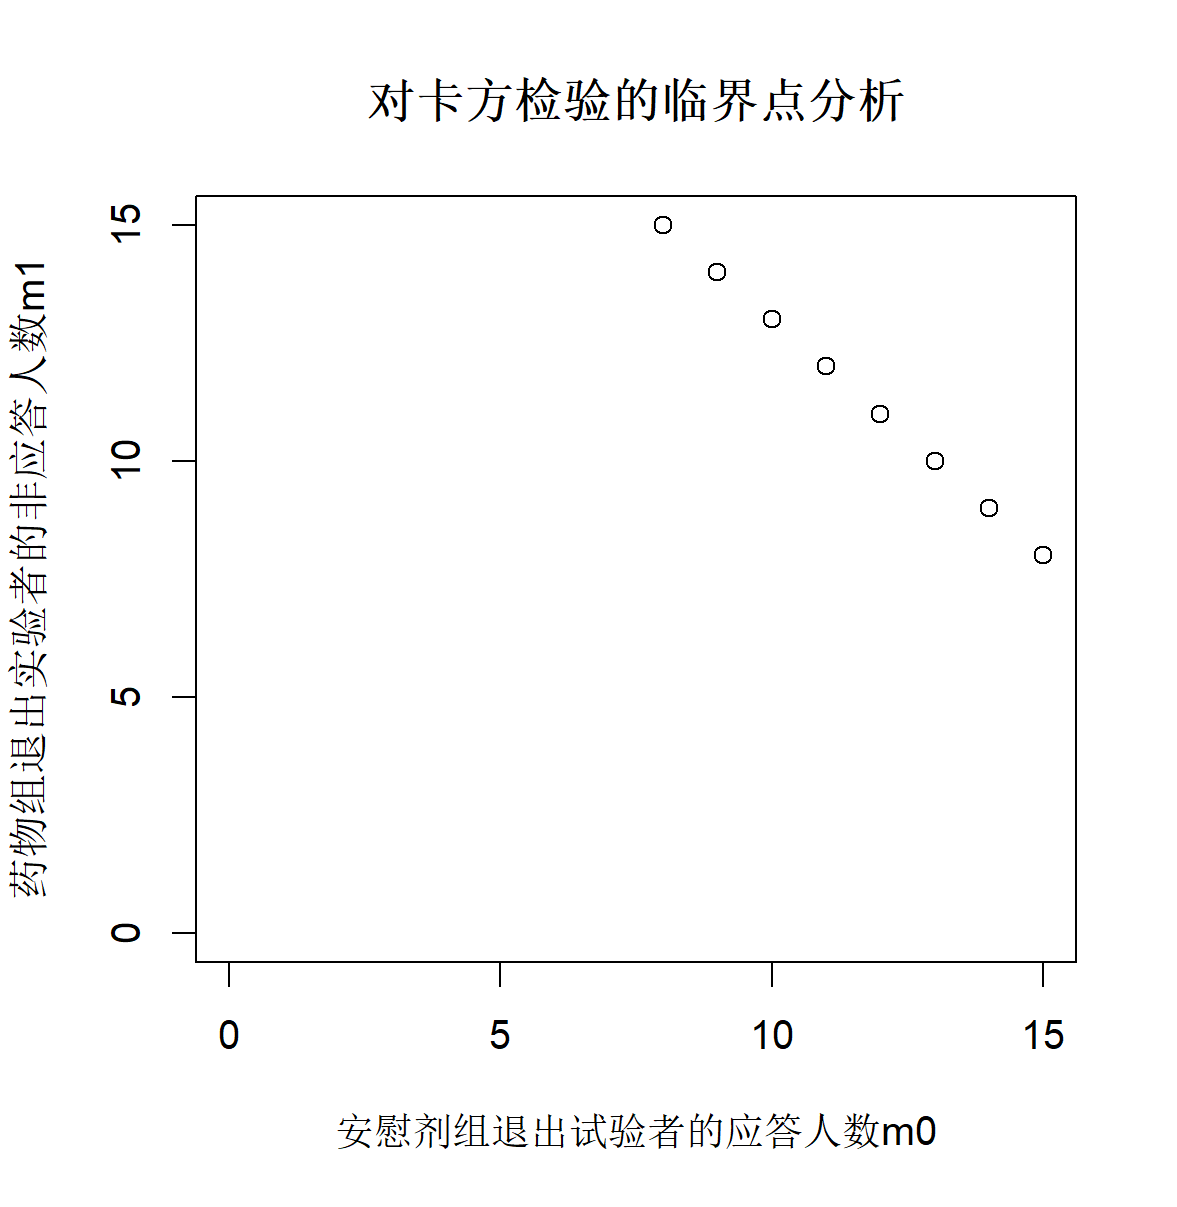
\includegraphics[width=0.49\textwidth]{image//tpa_chi.png}}
    \,    % 重点就在这,优先横向排列,自动换行
    \subfigure[对95$\%$置信区间是否包含0的临界点分析]
    {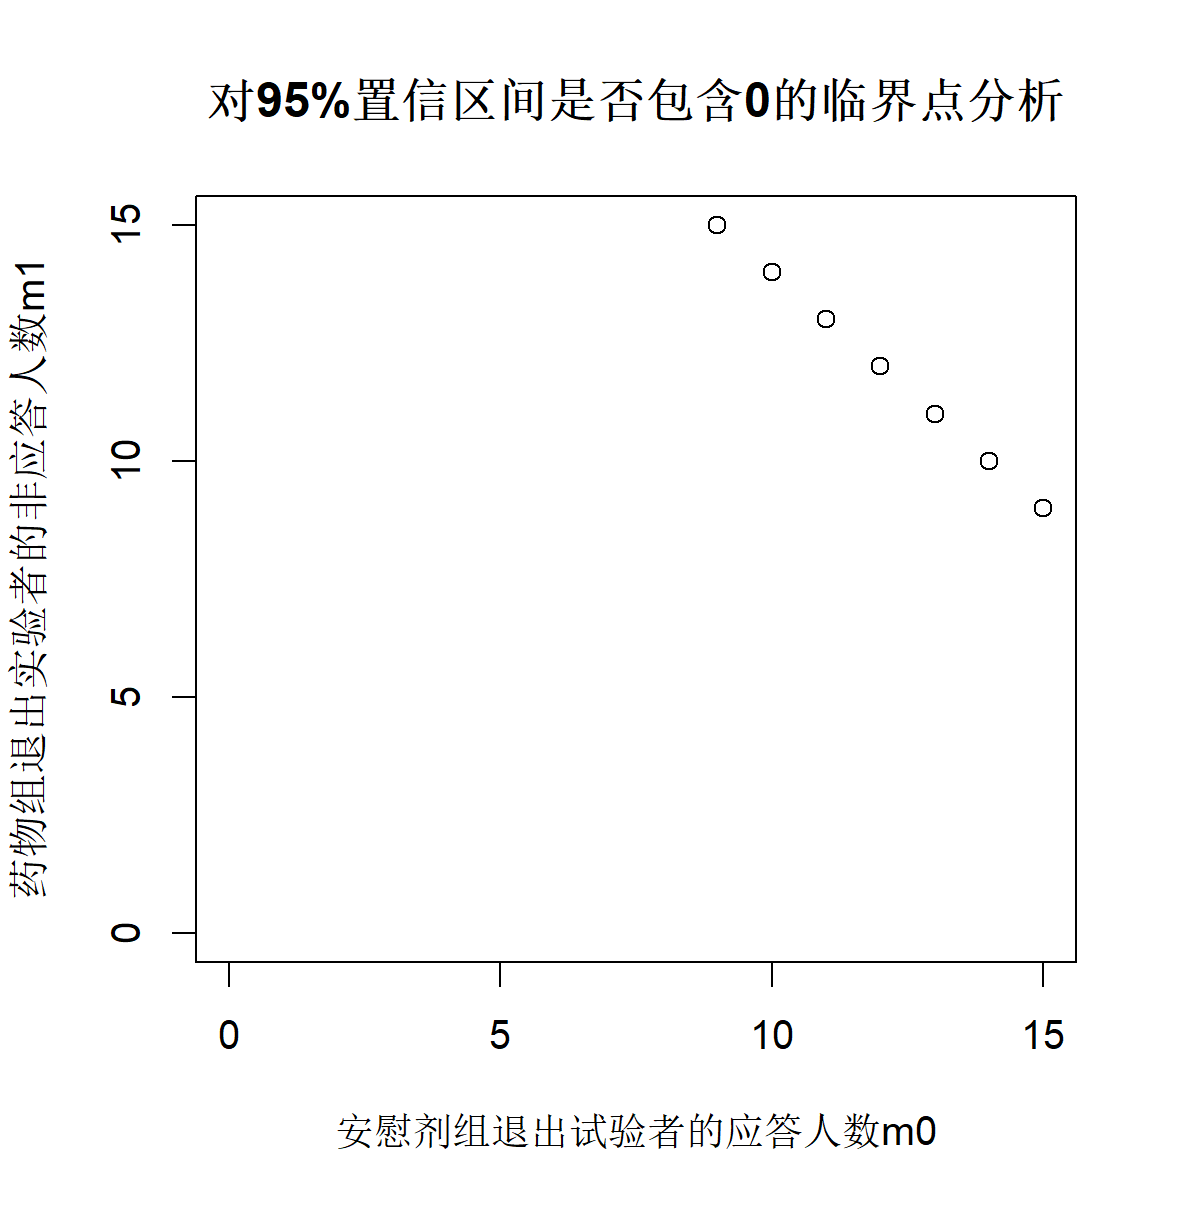
\includegraphics[width=0.49\textwidth]{image//tpa_CI.png}}
    \caption{临界点分析}
\end{figure}
图中点即为对应检验的结果发生反转的临界点。可以看出基本分布在一条直线上。
在这条直线左下方的范围内,检测结果不变。也即在大部分取值情况下,
检验结果与原分析结果是一致的,这说明了原分析结果具有稳健性,
也说明缺失数据对分析结果的影响较小。

\section{问题二}
\subsection{问题2.1}
在以下讨论中,我们仅考虑平衡设计,即两组样本量相等情况。此外,我们认为对于三个终点的讨论,都建立在
脱落率(即中途停止治疗的受试者比例)都为15$\%$的假设下。
\paragraph{样本量估计}
原假设和备择假设分别为:
\begin{align*}
    &H_0: \, \pi_1 - \pi_0 = 0\\
    &H_1: \,\pi_1 - \pi_0 > 0
\end{align*}

设单侧检验一类错误概率为$\alpha=0.025$,二类错误概率为$\beta=0.05$,
药物组$\pi_1=0.55$,安慰剂组$\pi_0=0.3$,在不考虑脱落的情况下,
可以得到总样本量(两组样本量之和)为:
\begin{align*}
    n &= 2\frac{(Z_{1-\alpha}+Z_{1-\beta})^2}{(\pi_1-\pi_0)^2}\left[\pi_1(1-\pi_1)+\pi_0(1-\pi_0)\right]\\
      &= 2\frac{(1.96+1.64)^2}{(0.55-0.30)^2}\left[ (0.55(1-0.55)) + 0.30(1-0.30) \right]\\
      &= 189.8
\end{align*}
向上取整得到$n=190$

设脱落率为$\eta=0.15$,则考虑脱落率后的样本量应该为:
\begin{equation*}
    n^* = \frac{n}{1-\eta} = \frac{190}{1-0.15} = 223.5
\end{equation*}
向上取整得到$n^* = 224$.

\paragraph{计算次要终点的把握度}
我们仍假设脱落率为$\eta=0.15$,则应取考虑脱落后的总样本量$n=190$进行计算。
对于第一个次要终点,原假设和备择假设分别为:
\begin{align*}
    &H_0: \, \mu_1 - \mu_0 = 0\\
    &H_1: \,\mu_1 - \mu_0 > 0
\end{align*}
设$\mu_1=0.65,\, \mu_2=0.35$,则两样本应答率之差的标准误为
\begin{align*}
    S &= \sqrt{\frac{\mu_1(1-\mu_1)}{n/2}+\frac{\mu_0(1-\mu_0)}{n/2}}\\
    &= \sqrt{\frac{0.65(1-0.65)}{95}+\frac{0.35(1-0.35)}{95}}\\
    &=0.0692
\end{align*}
统计量的单侧界值为
\[c=Z_{1-\alpha}S=1.96\times0.0692=0.1356\]
得到把握度为
\begin{align*}
    1-\beta &= \varPhi \left[\frac{\mu_1-\mu_0-c}{S}\right] \\
            &= \varPhi \left[\frac{0.65-0.35-0.1356}{0.0692}\right] \\
            & = 99.1\%
\end{align*}
其中$\varPhi(\cdot )$是标准正态分布的累积分布函数。

类似的,对于第二个次要终点,
设$\lambda_1=0.74,\, \lambda_2=0.50$,则两样本应答率之差的标准误为
\begin{align*}
    S &= \sqrt{\frac{\lambda_1(1-\lambda_1)}{n/2}+\frac{\lambda_0(1-\lambda_0)}{n/2}}\\
    &= \sqrt{\frac{0.74(1-0.74)}{95}+\frac{0.50(1-0.50)}{95}}\\
    &=0.0682
\end{align*}
统计量的单侧界值为
\[c=Z_{1-\alpha}S=1.96\times0.0682=0.13375\]
得到把握度为
\begin{align*}
    1-\beta &= \varPhi \left[\frac{\lambda_1-\lambda_0-c}{S}\right] \\
            &= \varPhi \left[\frac{0.74-0.50-0.13375}{0.0682}\right] \\
            & = 94.0\%
\end{align*}

\subsection{问题2.2}
\subsubsection{问题2.2.1}
根据陈建平等的研究\cite{陈建平2010期中分析的条件把握度及样本含量再估计},
我们决定基于布朗运动理论,估计条件把握度,再通过二分搜索法估计后一阶段所需样本含量。

该算法可以根据期中数据,计算条件把握度,如果把握度太低,则调整样本含量以达到期望把握度,如果
条件把握度较高,则建议提前结束临床试验。由于期中分析涉及到多重性问题,需要对一类错误进行控制。
Lan 和 DeMets提出了五类$\alpha$消耗函数\cite{陈峰2018临床试验统计学},可以根据具体情况选用其中一种。
在本算法中,我们采用了较为保守但总期望样本量较低的
O'Brien-Fleming消耗函数
\[\alpha(t)=1-\Phi(\frac{Z_{1-\alpha}}{\sqrt{t}})\]
对一类错误进行控制,其中$t$是信息时间。

该算法输入为:试验前预计总样本量$N$,已完成的样本量$n$,试验允许的最大样本量$N_{\text{max}}$,
两组各自的应答率$\eta_0,\eta_1$,
总的单侧检验显著性$\alpha$(默认为0.025),把握度$1-\beta$(默认为0.95),
迭代中止标准$tol$(即条件把握度与期望把握度的最大容忍误差)。
该算法输出包括如下四种情况:
\begin{enumerate}
    % \item 重估样本量小于等于已完成样本量$n$,可以结束试验,有效终止。
    \item 重估样本量大于试验允许最大样本量$N_{\text{max}}$,结束试验,无效终止,试验失败。
    \item 给出介于$n$和$N_{\text{max}}$的重估样本量$N'$。
    \item $tol$设置过小,无法满足二分法迭代停止准则,需重新设置。
\end{enumerate}

设计算法时采用的统计原理以及具体算法步骤请参考附件1,完成该算法的Python代码请参考附件2。

\subsubsection{问题2.2.2}
如果在实际临床试验中通过样本量重估的样本量小于实际预设定的样本量,应按照下述步骤处理:
\begin{itemize}
    \item 首先,检查样本量重估的过程是否有误,
        包括数据清洗过程中是否出现漏误,算法和代码是否合理,是否考虑了分层随机化与多中心因素,
        以及是否考虑排除数据中的离群值。
    \item 其次,如果以上诸检查均无误,应该向独立数据监察委员会汇报结果。
    \item 然后,根据陈峰和夏结来等人的专著\cite{陈峰2018临床试验统计学},
        当新样本量小于等于已完成的样本量$n$时,则可以提前终止试验;
        但当新样本含量小于原计划的样本量但大于已完成的样本量$n$,
        为确保试验的把握度,我们仍然会建议采用方案原计划的样本量。
    \item 若IDMC决定采用新样本量,则在最终分析时,应该在统计报告中详细说明样本量重估的过程、结果与可能影响。
\end{itemize}

\subsection{问题2.3}
此处仅考虑对两组应答率之差的单侧Wald检验方法。
设信息时间为$\tau' = \frac{n}{N'}$,其中$N'$是重估后的样本量。
根据陈建平等人的研究\cite{陈建平2010期中分析的条件把握度及样本含量再估计},
在进行最终分析时,需要考虑期中分析带来的一类错误膨胀问题。
这里我们与上文一致,仍采用五种类型消耗函数中的
O'Brien-Fleming消耗函数
$\alpha(\tau)=1-\Phi(\frac{Z_{1-\alpha}}{\sqrt{t}})$
(当然,也可以替换为其他消耗函数,只需要与期中分析时采用的类型保持一致即可)。
最终分析的显著性水平应该设置为$\alpha_2 = 0.025-\alpha(\tau')$.

那么,最终分析的单侧界值则相应变为$c' = Z_{1-\alpha_2}$,也即当
\[ \frac{P_1-P_0}{S}>Z_{1-\alpha_2}\]时,可以拒绝原假设,认为药物组应答率高于安慰剂组,
并且仍然能把一类错误率控制在单侧0.025的水平上。


\section{问题三}
\subsection{问题3.1}
我们决定采用回退法(fallback)进行多重性假设检验,考虑$\alpha_i$的回收与分配后,
以graphical approach方法展示假设检验的流程如下:

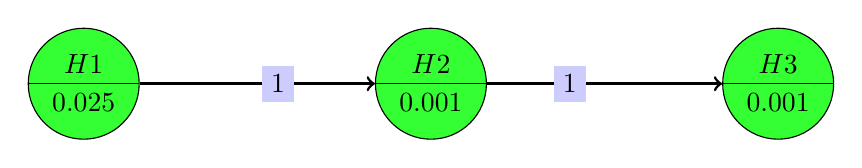
\begin{tikzpicture}
    \node (H1) at (75bp,-175bp)[draw,circle split,fill=green!80] {$H1$ \nodepart{lower} $0.025$};
    \node (H2) at (200bp,-175bp)[draw,circle split,fill=green!80] {$H2$ \nodepart{lower} $0.001$};
    \node (H3) at (325bp,-175bp)[draw,circle split,fill=green!80] {$H3$ \nodepart{lower} $0.001$};
    \draw [->,line width=1pt] (H1) to (145bp, -175bp) node[fill=blue!20] {$1$} to (H2);
    \draw [->,line width=1pt] (H2) to (250bp, -175bp) node[fill=blue!20] {$1$} to (H3);
\end{tikzpicture}

在该检验中,在初始时分配$\alpha_1=0.023,\alpha_2=0.001,\alpha_3=0.001$,
并在拒绝上一个假设后,将所有的$\alpha$值都传递给下一个假设。

我们提出该多重性假设检验方法的合理性如下:
\begin{enumerate}
    \item 主要终点假设检验重要性最高,故将其作为第一个假设进行检验。
    \item 由于可以进行$\alpha$的回收与分配,故使用贪心算法的思想,
        在初始时即让$\alpha_1$达到在$\alpha_i>0.001$约束下的最大值,也即$\alpha_1=0.023$。
        当主要终点的原假设被拒绝后,这部分显著性水平可以被全部传递到下一个假设,使下一个假设也更容易被拒绝。
    \item 初始时三个假设所分配的显著性水平相加正好为0.025,故该检验流程能将总的一类错误控制在单侧0.025。
    \item 每个终点的原假设被拒绝后,都将该终点的所有显著性水平传递给下一个终点,这样能够尽可能地穷耗总的$\alpha$。
    \item 根据问题2.1里的计算结果,第一个次要终点的把握度高于第二个次要终点,
        也即第一个次要终点的原假设更可能被拒绝。因此先检验第一个次要终点,再检验第二个次要终点,
        更有可能让两个次要终点的原假设都被拒绝,增加该药获批上市的可能性。
\end{enumerate}

\subsection{问题3.2}
在问题3.3中,根据我们提出的graphical approach方法,将显著性水平设置为单侧$\alpha_1=0.023$。
同样使用问题2.1中的样本量计算公式,可以得到:
\begin{align*}
    n &= 2\frac{(Z_{1-0.023}+Z_{1-0.05})^2}{(\pi_1-\pi_0)^2}\left[\pi_1(1-\pi_1)+\pi_0(1-\pi_0)\right]\\
      &= 2\frac{(1.995+1.64)^2}{(0.55-0.30)^2}
        \left[ (0.55(1-0.55)) + 0.30(1-0.30) \right]\\
      &= 193.4
\end{align*}
向上取整得到$n=194$

设脱落率为$\eta=0.15$,则考虑脱落率后的样本量应该为:
\begin{equation*}
    n^* = \frac{n}{1-\eta} = \frac{194}{1-0.15} = 228.2
\end{equation*}
向上取整得到$n^* = 229$.
\subsection{问题3.3}
在进行其中分析后,graphical approach的思想仍然是适用的,但需要对上述的多重假设检验流程进行修改,
在主要终点的检验之前再增加一个代表期中分析的节点,并同样利用$\alpha$消耗函数,将总一类错误概率
分配一部分给期中分析。此外,在期中分析之后,不会把期中分析$\alpha$传递给最终检验。示意图如下:

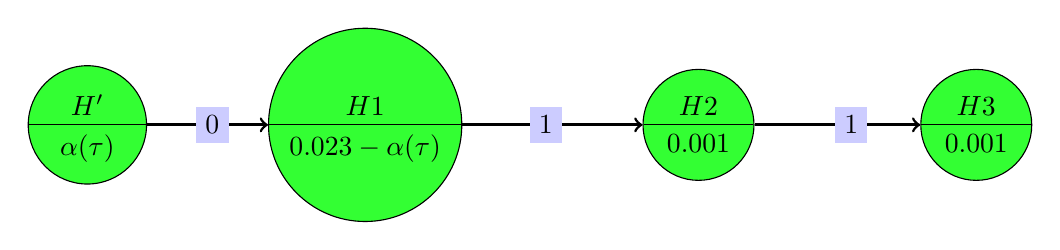
\begin{tikzpicture}

    \node (H') at (25bp,-275bp)[draw,circle split,fill=green!80] {$H'$ \nodepart{lower} $\alpha(\tau)$};
    \node (H1) at (125bp,-275bp)[draw,circle split,fill=green!80] {$H1$ \nodepart{lower} $0.023-\alpha(\tau)$};
    \node (H2) at (245bp,-275bp)[draw,circle split,fill=green!80] {$H2$ \nodepart{lower} $0.001$};
    \node (H3) at (345bp,-275bp)[draw,circle split,fill=green!80] {$H3$ \nodepart{lower} $0.001$};
    \draw [->,line width=1pt] (H') to (70bp, -275bp) node[fill=blue!20] {$0$} to (H1);
    \draw [->,line width=1pt] (H1) to (190bp, -275bp) node[fill=blue!20] {$1$} to (H2);
    \draw [->,line width=1pt] (H2) to (300bp, -275bp) node[fill=blue!20] {$1$} to (H3);
\end{tikzpicture}
    
其中,$H'$代表了期中分析,$\tau$是信息时间,$\alpha(\tau)$是某个预先选取的$\alpha$消耗函数,并且需要满足
$0.023-\alpha(\tau)>0.001$。


\section{问题四}
% 根据研究方案中的访视要求,受试者从第0周(即首次给药)开始
% 每隔4周会被要求到研究中心进行给药并定期检查用以评估药物的安全性并对上述三个终点有测量,
% 直至24周研究结束或者受试者提前退出研究。
% 请阐述如何考虑将上述重复测量的数据用于问题1.2中的分析中,
% 并应用到附件中的试验数据。请阐述该分析方法的结果和问题1.4所得的结果是否有差异。
% 如果有,请具体说明。 
对于重复测量数据,不同时间点的测量数据之间存在相关性,
且中途部分受试者退出,造成部分数据缺失,这使得我们无法使用传统的方差分析。
我们认为,对于上述的问题,可以使用广义估计方程(GEE)进行模型拟合,该模型有较稳健且一致的估计。
此外,我们推测组别和测量时间之间很可能具有交互效应,
也即药物组和安慰剂组的应答率随时间的增加具有不同的变化趋势。
因此,还可以在GEE中引入组别和时间的交互项。下面,我们仍以主要终点为例,对附件中的试验数据建模,
有关的R代码与建模结果如下:
\lstinputlisting[style = R,
caption={以主要终点为例,对重复测量数据用GEE进行建模},
label = {gee}]{codes//gee.R}

注意到该模型的地区变量的系数(Europe:0.74763,North America:0.05581)和问题1.4中
只用第24周未缺失数据进行多元逻辑回归(逐步回归)所得到的地区变量系数
(Europe:0.77835,North America:-0.03275)整体上一致,这反映出了GEE模型的稳健性和一致性。

但是,在引入时间和分组的交叉项之后,分组变量的系数变为0.39443994,与问题1.4中
所得到的分组变量系数1.04392有较大差异,这反映出时间与分组之间存在比较明显的交互作用,
可以看作原本的分组变量引起的效应,被进一步拆解为独立效应和交互效用。
这也说明了两组的应答率随时间的变化趋势不同。

此外,如果将该模型的分组变量,以及分组与第24周的交互项的系数相加,
即$0.57184144+0.39443994 =0.96628138$,发现该值与问题1.4中得到的分组变量系数1.04392较为接近,
说明在使用GEE进行分析后,将分组变量的独立效应和与时间的交互效应相加,
基本与不考虑时间因素所得到的分组变量效应相一致,这同样说明了GEE模型的稳健性和一致性。




\bibliographystyle{plain}
\bibliography{ref}

\section*{附录:正文与附录中均未包含的代码}
\subsection*{临界点分析所使用的R代码}

\lstinputlisting[style = R,
caption={临界点分析所使用的R代码},
label = {tpa}]{codes//tipping_point.R}


\end{document}


% \begin{figure}[H]
%     \centering  %图片全局居中
%     \includegraphics[width=0.8\textwidth]{result3}
%     \caption{The heap after performing INCREASE-KEY(A, 10, 28)}
% \end{figure}